\documentclass{article}
\usepackage{graphicx}
\usepackage{geometry}
\geometry{a4paper, margin=1in}

\begin{document}

\title{Heart Data Analysis}
\author{}
\date{}
\maketitle

\section{Data Table}
\input{heart_table} % if you generated this separately

\section{Plots}

\subsection{Histogram of Gender vs. Heart Disease}
\begin{figure}[h!]
    \centering
    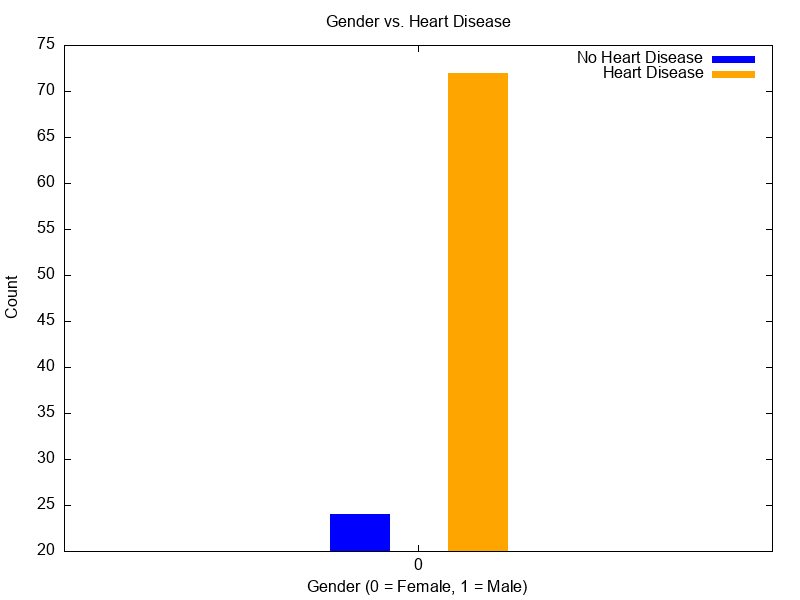
\includegraphics[width=0.7\textwidth]{gender_vs_heart_disease.png}
    \caption{Histogram showing the distribution of gender and heart disease cases.}
    \label{fig:gender_heart_disease}
\end{figure}

\subsection{Age vs Blood Pressure}
\begin{figure}[h!]
    \centering
    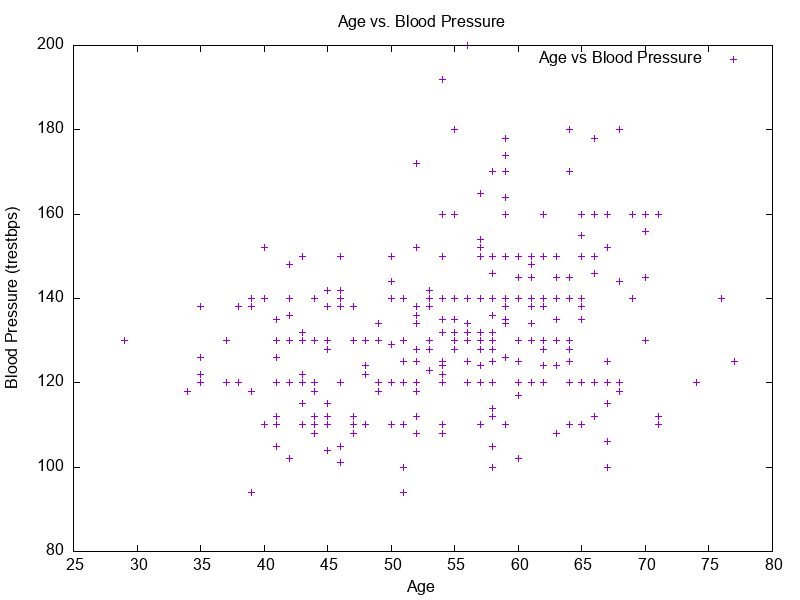
\includegraphics[width=0.7\textwidth]{age_vs_blood_pressure.png}
    \caption{Scatter plot of Age vs Blood Pressure.}
    \label{fig:age_blood_pressure}
\end{figure}

\subsection{Age vs Cholesterol (Non-Heart Disease)}
\begin{figure}[h!]
    \centering
    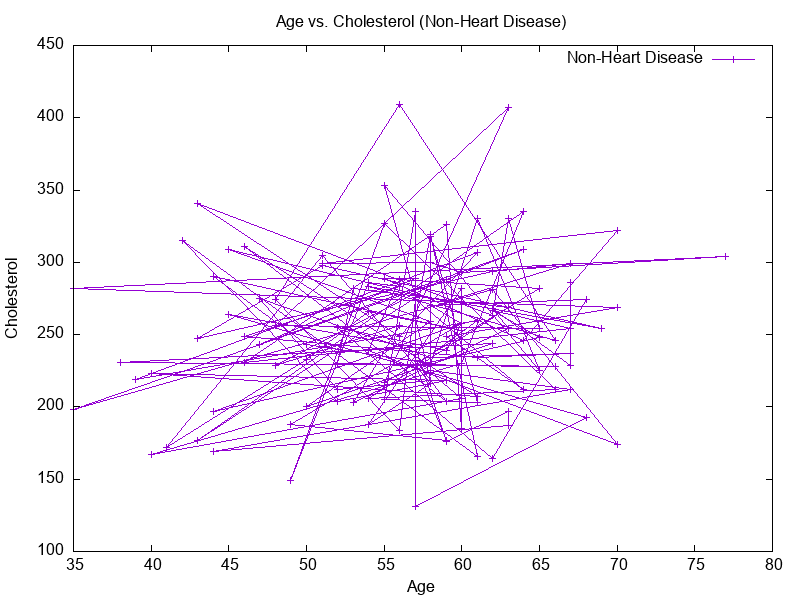
\includegraphics[width=0.7\textwidth]{age_vs_cholesterol_non_heart_disease.png}
    \caption{Age vs Cholesterol for patients without heart disease.}
    \label{fig:age_cholesterol_non_heart_disease}
\end{figure}

\subsection{Age Groups with Heart Disease}
\begin{figure}[h!]
    \centering
    \includegraphics[width=0.7\textwidth]{age_groups_heart_disease.png}
    \caption{Pie chart showing the percentage of age groups with heart disease.}
    \label{fig:age_groups_heart_disease}
\end{figure}

\end{document}
